\documentclass[letterpaper]{article}

\usepackage{listings}
\usepackage{color}
\usepackage{courier}
\usepackage{graphicx}

\lstset{ %
% language=Octave,                % choose the language of the code
basicstyle=\ttfamily,       % the size of the fonts that are used for the code
numbers=left,                   % where to put the line-numbers
numberstyle=\footnotesize,      % the size of the fonts that are used for the line-numbers
stepnumber=1,                   % the step betweeblog posn two line-numbers. If it's 1 each line
                                % will be numbered
numbersep=5pt,                  % how far the line-numbers are from the code
backgroundcolor=\color{white},  % choose the background color. You must add \usepackage{color}
showspaces=false,               % show spaces adding particular underscores
showstringspaces=false,         % underline spaces within strings
showtabs=false,                 % show tabs within strings adding particular underscores
frame=single,	                % adds a frame around the code
tabsize=2,	                % sets default tabsize to 2 spaces
captionpos=b,                   % sets the caption-position to bottom
breaklines=true,                % sets automatic line breaking
breakatwhitespace=false,        % sets if automatic breaks should only happen at whitespace
% title=\lstname,                 % show the filename of files included with \lstinputlisting;
%                                 % also try caption instead of title
escapeinside={\%*}{*)},         % if you want to add a comment within your code
morekeywords={*,...}            % if you want to add more keywords to the set
}

\begin{document}

% \section{Prerequisites}

% You might want to download latest Mapnik release (0.7.1) from here.
% There's also a set of geodata files which should be downloaded from here.
% For the most adventurous of you, download osm2pgsql from here and the OSM planet file from here.

\section{Cartography}
\label{sec:cartography}

\subsection{Definitions}
\label{sec:definitions}

\begin{description}
\item[GIS] Geographic Information System, a system that collects, analyzes, manages or processes in any other way data linked to location.
\item[Cartography] Study and making of maps in all their aspects.
\item[Map] Graphic representation of the geographical setting, a product of applying cartography rules to geographic data.
\end{description}

Cartography can be used for analyzing, representing, recording and understanding the interrelation of things tied to location. The fundamental function of cartography is to bring those things into view (i.e. making maps).

All maps are concerned with two elements of reality:
\begin{description}
\item[Locations] Positions in two-dimensional space (e.g. \textit{x, y} coordinates of places)
\item[Attributes] Qualities or magnitudes (e.g. languages, soil type, etc)
\end{description}

All geographical maps are \emph{reductions}, that is the map is smaller than the region it portrays.
The dimensional relationship between reality and the map is called \emph{scale}.

All maps involve geometrical transformations.
It is common to transform a spherical surface to surface that is easier to work with, such
as computer screen. Such transformations are called \emph{map projections}.

All maps are \emph{abstractions} over reality. Real world is complex and full of features, so that
putting even small part of it in image would make maps confusing.
Consequently, maps portray only the information that has been chosen to fit for
the use of the map.

To portray real features, all maps use \emph{signs} to stand for elements of reality. All signs consist of various kinds of marks, such as lines, dots, colors and so on. When using map, we must constantly compare the symbols with those in the legend.

\subsection{Categories of maps}
\label{sec:categories-maps}

Though the maps can come in millions of variations, there are some recognized ways of grouping
objectives and uses of maps, which allow us to catalog them to some degree. It's important to
note that these classifications are only conventional and thus a map can be easily
put in almost any class described here. The classification still gives a general idea
of what the said map was designed for.

\subsubsection{Classed by scale}
\label{sec:classed-scale}

\emph{Map scale} is the ratio between the dimensions of the map and those of reality.
When a large area is fitted into small view (e.g. map of the whole world), a map
is described as being \emph{small-scale map}. If a map is being used to show relatively
small territory (for example, less than 1 km$^{2}$), than it is described as
\emph{large-scale map}.

\subsubsection{Classed by function}
\label{sec:classed-function}

Depending on the objective of the map, we can group maps into following classes:
\begin{description}
\item[General reference maps] Maps that are created in order to show the locations
of a variety of different features, such water bodies, coastlines and roads.
\item[Thematic maps] Maps that are concentrated on the distribution of a single
attribute or the relationship among several others. For example, population
or average income maps can be classified at thematic.
\item[Charts] Maps designed to serve the needs of navigators.
\end{description}

\subsubsection{Classed by subject matter}
\label{sec:class-subj-matt}

It is sometimes useful to group maps on the basis of their subject matter.
There is no limit to the number of classes of maps that can be created by
grouping them according to their dominant subject matter.
Nevertheless, several important categories can be recognized:

\begin{description}
\item[Cadastral maps] The map that accompanies cadastre -- official list of
property owners and their land holdings.
\item[Plans] Detailed, commonly very large-scale maps, showing buildings, roadways, administrative
  boundaries.
\end{description}

\subsection{Map projections}

\begin{description}
\item[Map projection] Method of representing the surface of three-dimensional object on a plane.
\item[Reference globe] Hypothetical mapping of the earth to a globe of chosen size (scale)
\item[Principal scale] Representative fraction of the reference globe. Division of the earth's
  radius by the radius of the reference globe.
\item[Scale factor] Actual scale of the map divided by the principal scale. Will be 1.0 on the globe and will vary when mapped onto flat map.
\end{description}

\subsubsection{Tissot's indicatrix}
\label{sec:tissots-indicatrix}

\emph{Tissot's indicatrix} is a special graphic device, created in order to
illustrate the angular and areal distortions that occur when projecting the map.

The indicatrix itself is a point represented by an infinitely small circle with
a radius of 1.0. It can be shown that in any system of transformation the values
of \textit{a} and \textit{b} will differ from 1.0.

An example of indicatrix is shown below.

\begin{centering}
  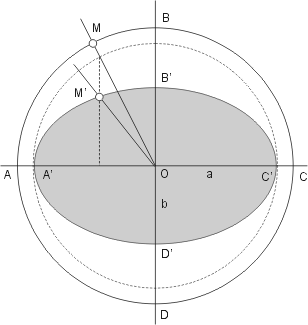
\includegraphics[scale=0.5]{indicatrix.png}
\end{centering}

Here you can see the circle (defined by center $O$ and points $ABCD$)
which represents the point. For this circle $OA = a = OB = b = 1.0$.

First, let's examine transformations of principal directions ($OA$ and $OB$)
We can that $OA' < OA$ as well as $OB' < OB$.
This shows the \emph{reduction} of scale factor.
A projection would be called \emph{conformal} if $OB' = OA'$.

The area distortion is apparent because $OA' \times OB' \neq 1$. If that
was the case, the projection would then be labeled as \emph{equal-area}.

Angle distortion can be seen when examining projection of the angle $MOA$ to
$M'OA'$. Because $MOA > M'OA'$ there is an angular distortion.


\subsubsection{Map distortions}
\label{sec:map-distortions}

When the surface of the globe is being projected to a flat surface
some transformation of the geometrical relations is guaranteed.
Here four important classes of distortion

\begin{description}
\item[Transformation of angles] At each point on the globe's surface (except for poles) the cardinal directions are orthogonal. When the projected map retains this characteristic, the projection
that was used is called \emph{conformal}.
\item[Transformation of areas] It is possible for a map projection to preserve the
representation of areas, so that each area is shown with correct relative size. Such
projection is called \emph{equal-area} or \emph{equivalent}. Note that it is not
possible for the projection to be both conformal and equivalent.
\item[Transformation of distances] For the distance between two points to maintain
  its scale the scale factor must be uniform for the entire extent of the line.
  In order to achieve that, we have to options
  \begin{itemize}
  \item Have a scale factor of 1.0 along one or more parallel lines. When this option
    chosen these lines are called \emph{standard lines} or \emph{standard parallels}.
  \item Have a scale factor of 1.0 along all lines from one or two selected points.
    The projection will then be called \emph{equidistant} and the point(s) will be called
    \emph{standard points}
  \end{itemize}
\item[Transformation of directions] A projection that retains the directions can be
  described as a projection that shows all great circles as straight lines. If we want
  to keep this property for all points on the map, \emph{gnomonic} projection is used.
  Unfortunately, such projections can only be used for limited areas. The other approach
  is to use projection that can show correct great circles from only one or two points.
  Such projection is called \emph{azimuthal}.
\end{description}

\pagebreak

\section{Mapnik}
\label{sec:mapnik}

\begin{description}
\item[Mapnik] Rendering library, created specifically for OpenStreetMap which later grew
  into general cartography framework.
\end{description}

\subsection{Rendering with pure Python}
\label{sec:rendering-with-pure}

\begin{figure}[h]
  \centering
  \lstinputlisting[language=Python]{simple.py}
  \caption{Hello world with Mapnik}
  \label{fig:1}
\end{figure}

\subsection{Python for code, XML for configuration}
\label{sec:python-code-xml}

\begin{figure}[h]
  \centering
  \lstinputlisting[language=Python]{simple_xml.py}
  \caption{Ofsetting work to XML}
  \label{fig:hw-py}
\end{figure}

\begin{figure}[h]
  \centering
  \lstinputlisting[language=XML]{simple.xml}
  \caption{Hello world with XML}
  \label{fig:hw-xml}
\end{figure}

\begin{figure}[h]
  \centering
  \lstinputlisting[language=Python]{simple_almost_fixed.py}
  \caption{Fixing rendering}
  \label{fig:hw-py-almost-fixed}
\end{figure}

\begin{figure}[h]
  \centering
  \lstinputlisting[language=Python]{explaining_bounds.py}
  \caption{Explaining bounds}
  \label{fig:hw-py-corrected-and-explaining}
\end{figure}

\begin{figure}[h]
  \centering
  \lstinputlisting[language=Python]{simple_fixed.py}
  \caption{Correcting bounds}
  \label{fig:hw-py-corrected}
\end{figure}

\begin{figure}[h]
  \centering
  \lstinputlisting[language=Python]{projecting_coords.py}
  \caption{Explaining bounds}
  \label{fig:hw-py-projecting-coords}
\end{figure}

\begin{figure}[h]
  \centering
  \lstinputlisting[language=Python]{simple_refactored.py}
  \caption{Refactoring Mapnik code}
  \label{fig:hw-refactoring}
\end{figure}

\subsection{Adding more meat to XML}
\label{sec:adding-more-meat}

\begin{figure}[h]
  \centering
  \lstinputlisting[language=XML]{countries.xml}
  \caption{Adding more to XML}
  \label{fig:xml-more}
\end{figure}

\begin{figure}[h]
  \centering
  \lstinputlisting[language=XML]{roads.xml}
  \caption{Adding roads to XML}
  \label{fig:xml-roads}
\end{figure}

\begin{figure}[h]
  \centering
  \lstinputlisting[language=XML]{roadnames.xml}
  \caption{Adding road names to XML}
  \label{fig:xml-road-names}
\end{figure}

\begin{figure}[h]
  \centering
  \lstinputlisting[language=XML]{polygons.xml}
  \caption{Adding buildings and parks}
  \label{fig:xml-polygons}
\end{figure}

\begin{figure}[h]
  \centering
  \lstinputlisting[language=XML]{zooms.xml}
  \caption{Adding zoom levels}
  \label{fig:xml-zooms}
\end{figure}

% \section{Rendering}

% \subsection{Perception}

% In case with cartography a careful approach is preferred when choosing
% color scheme. Not only color outlines main features of the map, but also
% helps achieve the goal of being accessible for everybody.

% \subsection{Simple Mapnik rendering}

% This is a short example which creates basic map object, applies simple styling
% rules and provides a datasource.

% \lstinputlisting{simple-rendering.py}

% Let's outline several points here.

% Creation of map

% Creating and applying styles

% Attaching datasources

% Rendering

% \subsection{Simple Mapnik XML}

% Of course, defining such logic in code is not only cumbersome, but also makes
% such tasks as serialization and changing Mapnik styles on the fly

% \lstinputlisting{simple.xml}

% IMAGE

% Adding Tissot's indicatrix

% \lstinputlisting{tissot-indicatrix.xml}

% IMAGE

% Viewing in different projection

% \lstinputlisting{tissot-indicatrix-mercator.xml}

% IMAGE

% \lstinputlisting{tissot-indicatrix-mercator.xml}

% IMAGE



\section{References}

% On projections and srs
% http://www.sharpgis.net/post/2007/05/Spatial-references2c-coordinate-systems2c-projections2c-datums2c-ellipsoids-e28093-confusing.aspx
% http://spatialreference.org/
% http://proj.maptools.org/gen_parms.html
% http://trac.osgeo.org/proj/wiki/GenParms
% http://trac.mapnik.org/wiki/IntroductionToGIS
% http://en.wikipedia.org/wiki/Winkel_Tripel_projection



\end{document}
